% Two stages of the Smith--Volterra--Cantor set. Charcoal bars remain; coral marks a removed open middle.
% Stage 1 removes an open interval of length 1/4. Stage 2 removes an open interval of length 1/16 from each surviving bar.
\begin{tikzpicture}[x=11.2cm,y=1cm,line cap=round]
  % Stage 1
  \fill[MidnightBlue] (0,1.55) rectangle (0.375,2.05);
  \fill[MidnightBlue] (0.625,1.55) rectangle (1,2.05);
  \draw[BurntOrange,line width=1.6pt] (0.390,1.80)--(0.610,1.80);
  \node[font=\footnotesize,text=BurntOrange] at (0.50,2.28) {open gap of length $\tfrac14$};
  \node[font=\footnotesize,text=MidnightBlue,anchor=west] at (0,1.28) {stage $1$};
  \node[font=\footnotesize,text=MidnightBlue,anchor=north] at (0.1875,1.50) {$[0,\tfrac38]$};
  \node[font=\footnotesize,text=MidnightBlue,anchor=north] at (0.8125,1.50) {$[\tfrac58,1]$};
  % Stage 2
  \fill[MidnightBlue] (0,0.15) rectangle (0.15625,0.65);
  \fill[MidnightBlue] (0.21875,0.15) rectangle (0.375,0.65);
  \fill[MidnightBlue] (0.625,0.15) rectangle (0.78125,0.65);
  \fill[MidnightBlue] (0.84375,0.15) rectangle (1,0.65);
  \draw[BurntOrange,line width=1.6pt] (0.168,0.40)--(0.207,0.40);
  \draw[BurntOrange,line width=1.6pt] (0.390,0.40)--(0.610,0.40);
  \draw[BurntOrange,line width=1.6pt] (0.793,0.40)--(0.832,0.40);
  \node[font=\footnotesize,text=MidnightBlue,anchor=west] at (0,-0.12) {stage $2$};
  \node[font=\footnotesize,text=BurntOrange,anchor=west] at (1.02,0.40) {gaps of length $\tfrac1{16}$};
  % A later punch, drawn on the first surviving bar
  \draw[BurntOrange,dashed] (0.07,0.65)--(0.07,0.98);
  \draw[BurntOrange,dashed] (0.09,0.65)--(0.09,0.98);
  \node[font=\footnotesize,text=BurntOrange,anchor=west] at (0.12,0.98) {the next stage cuts this bar too};
\end{tikzpicture}
